%+----------------------------------------------------------------------------+
%| SLIDES: 
%| Chapter: Complementary material - details on eventual questions
%| Author: Antonio miti
%| Event: PHD preliminary Defence
%+----------------------------------------------------------------------------+
%- HandOut Flag -----------------------------------------------------------------------------------------
\makeatletter
\@ifundefined{ifHandout}{%
  \expandafter\newif\csname ifHandout\endcsname
}{}
\makeatother

%- D0cum3nt ----------------------------------------------------------------------------------------------
\documentclass[beamer,10pt]{standalone}   
%\documentclass[beamer,10pt,handout]{standalone}  \Handouttrue  

\ifHandout
	\setbeameroption{show notes} %print notes   
\fi

	
%- Packages ----------------------------------------------------------------------------------------------
\usepackage{custom-style}

%--Beamer Style-----------------------------------------------------------------------------------------------
\usetheme{toninus}



\providecommand{\blank}{\text{\textvisiblespace}}


\newcommand{\subsectiontitle}{
  \begin{frame}
  \vfill
  \centering
  \begin{beamercolorbox}[sep=8pt,center,shadow=true,rounded=true]{title}
    \usebeamerfont{title}\insertsectionhead\par%
    \usebeamerfont{title}\insertsubsectionhead\par%
  \end{beamercolorbox}
  \vfill
  \end{frame}
}

\providecommand{\blank}{\text{\textvisiblespace}}




%---------------------------------------------------------------------------------------------------------------------------------------------------
%- D0cum3nt ----------------------------------------------------------------------------------------------------------------------------------
\begin{document}
%------------------------------------------------------------------------------------------------

%##################################################################################
\begin{frame}
	\begin{center}
	\Huge\emph{Supplementary Material}
	\end{center}
\end{frame}
\note[itemize]{
	\item
}
\addtocounter{framenumber}{-1}
%##################################################################################





%===================================================================================
\section{Background}
%===================================================================================



%-------------------------------------------------------------------------------------------------------------------------------------------------
\subsection{Symplectic Manifolds}
%-------------------------------------------------------------------------------------------------------------------------------------------------


%------------------------------------------------------------------------------------------------
\begin{frame}{Geometry of symmetries}\label{frame:geometrysymmetries}
	Basic mechanical structures are encoded in geometry. but there is another complementary geometrical property that's natural in physics: symmetry!
	\begin{alertblock}{Upshot}
		Continous symmetries are described by actions of a Lie group on $M$.
	\end{alertblock}
	\begin{block}{Noether}
		Presence of symmetries $\quad \Rightarrow \quad$ existence of conserved quantities.
	\end{block}	
	\begin{block}{Key concept:}
		Noether current are encoded in a \emph{moment map}  $\mu :M \rightarrow \mathfrak{g}^*$ (the dual of the comoment map $f$. 
	\end{block}
  \begin{columns}[T]
   	\begin{column}{.6\textwidth}
			\begin{block}{Symplectic reduction:}
			\begin{itemize}
				\item System dynamics should be restricted to level set of conserved observables in order to efficiently store dynamical properties.
				\item Under certain assumptions, $\mu^{-1}( 0 )/G$ is a symplectic manifold with an "induced" symplectic structure.
			\end{itemize}
			\end{block}
    \end{column}
    \begin{column}{.4\textwidth}	
			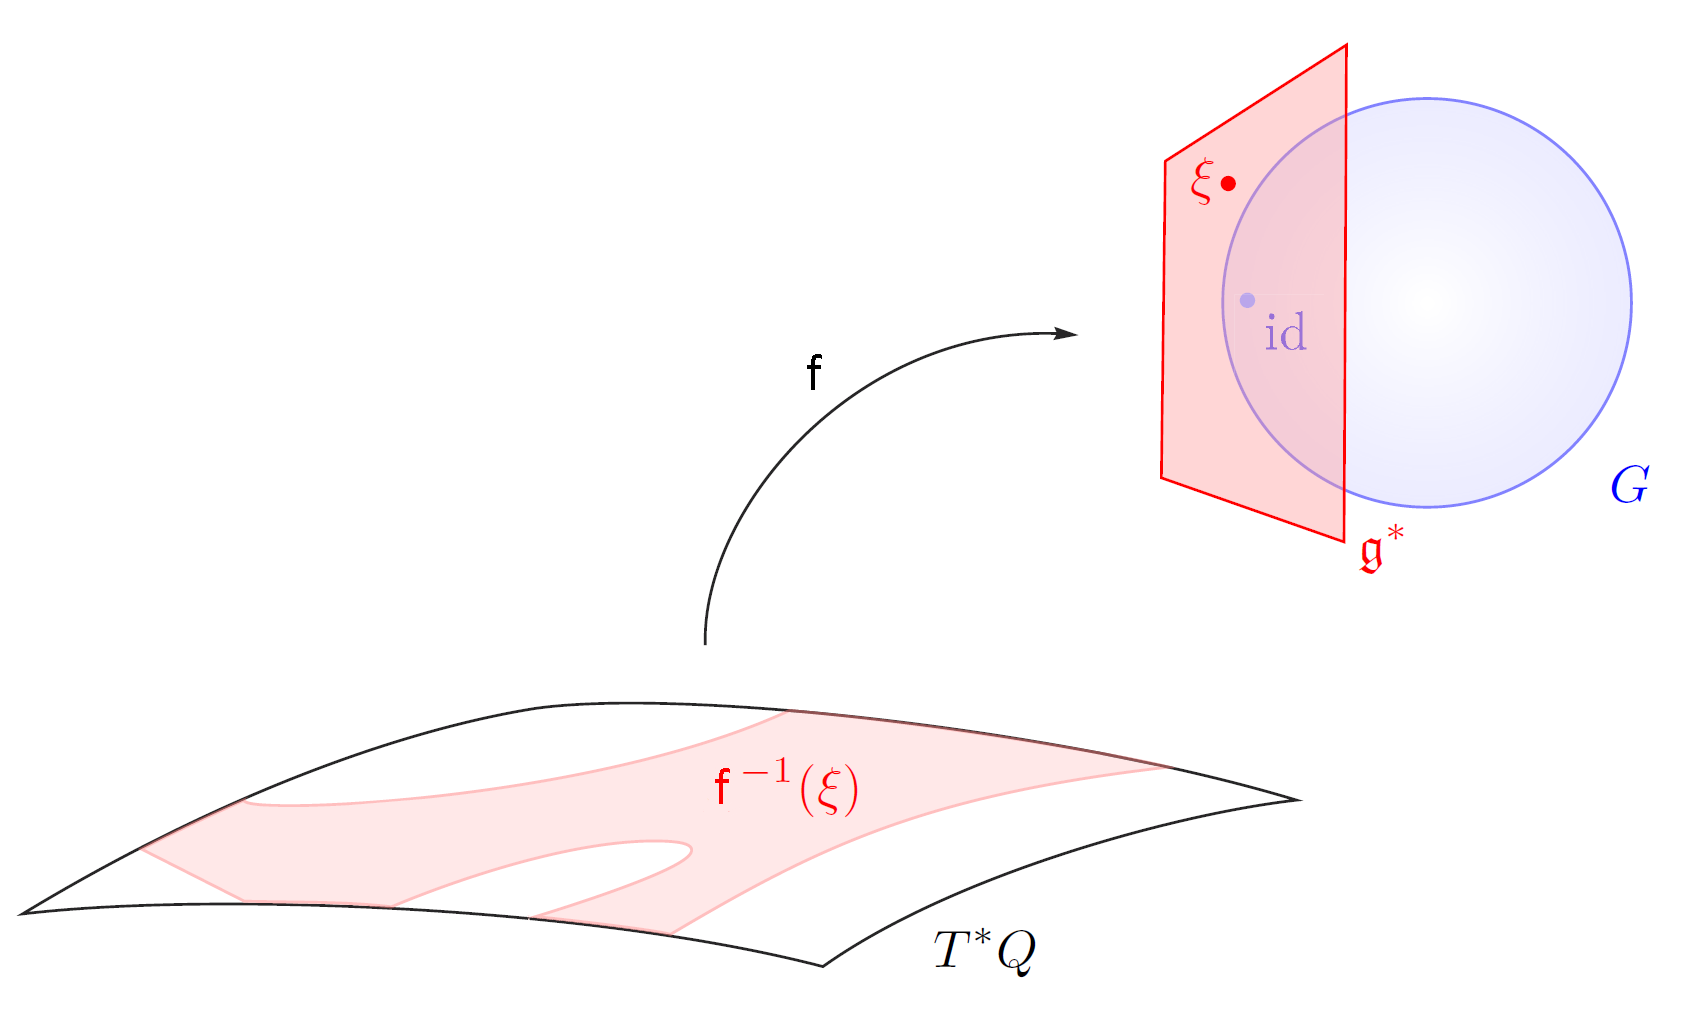
\includegraphics[width=\textwidth]{Pictures/Reduction} 
  	\end{column}
	\end{columns}			
\end{frame}
\note[itemize]{
	\item
}
%------------------------------------------------------------------------------------------------

%----------------------------------------------------------------------------------------------------------------------------------
\begin{frame}[fragile]{Configuration Space}
  	\begin{columns}[T]
    	\begin{column}{.5\textwidth}		
			\includegraphics<1>[width=\textwidth]{Pictures/GeoMec}
			\includegraphics<2->[width=\textwidth]{Pictures/GeoMec_noted}
    	\end{column}
    	\begin{column}{.5\textwidth}
			\begin{displaymath}				
   				Q \coloneqq
   				\left\{
				\parbox{45mm}{All possible admissible spatial displacements of a system.}
				 \right\}.
			\end{displaymath}

			\begin{block}<2->{Assumption 1:}
				For point particle $Q$ is a submanifold of $\mathbb{R}^n$.
			\end{block}

			\begin{block}<3->{Assumption 2:}
				Constraints are intrinsically encoded in the geometric structure of $Q$.
			\end{block}

			\vfill
			\begin{alertblock}<4->{Upshot:}
				$Q$ is a \emph{smooth manifold}. 
				Configuration of a system are naturally described by points on it. Configuration coordinates are charts.
			\end{alertblock}
    	\end{column}
  	\end{columns}	
\end{frame}
\note[itemize]{
	\item Consider the set of all possible admissible spatial displacements of a system.
}
%----------------------------------------------------------------------------------------------------------------------------------



%----------------------------------------------------------------------------------------------------------------------------------
\begin{frame}[t]{Symplectic Geometry}
	\begin{exampleblock}{Key point}
		$T^\ast Q$ it's naturally symplectic (i.e. endowed with a closed, bilinear, skew-symmetric form).
		\\
		\underline{Abstraction}: Mechanical systems $\quad \mapsto \quad$ symplectic manifold $(M,\omega)$.
	\end{exampleblock}
	%
	\vfill
  	\begin{columns}[T]
    	\begin{column}{.5\textwidth}	
			\includegraphics<1>[width=1.1\textwidth]{Pictures/Fig7} 
			\includegraphics<2->[width=1.1\textwidth]{Pictures/Fig8} 		
    	\end{column}
    	\begin{column}{.5\textwidth}
			\begin{itemize}
				\item<1-> Classical observables are elements in $C^\infty(M,\mathbb{R})$
				\item<2-> Observable yields hamiltonian fields $\textrm{d} H = \omega(X_H, \cdot)$
				\item<3-> Trajectories are integral flows of $X_H$
			\end{itemize}
    	\end{column}
  	\end{columns}				
	%
\end{frame}
\note[itemize]{
	\item

}
%----------------------------------------------------------------------------------------------------------------------------------

	\begin{frame}{Trajectories}
  	\begin{columns}[T]
    	\begin{column}{.5\textwidth}		
				\begin{center}
					Double Pendulum:
  	  				\includegraphics<1->[width=\textwidth]{Pics/Fig4} 
    				\vspace{3em}
    				General system:
					\includegraphics<1->[width=\textwidth]{Pics/Fig2} 	
				\end{center}
    	\end{column}
    	\begin{column}{.5\textwidth}


 				\begin{alertblock}<2->{Upshot}
 					 Trajectories of the system can be described by smooth parametrized curves on $Q$
 					\begin{displaymath}
 						Conf = C^\infty(\mathbb{R},Q)
 					\end{displaymath}
 				\end{alertblock}
 					\vspace{1em}

					
    	\end{column}
  	\end{columns}	
	\end{frame}

	\begin{frame}{Velocities}
  	\begin{columns}[T]
    	\begin{column}{.5\textwidth}		
				\begin{center}
					Double Pendulum:
  	  				\includegraphics<1->[width=\textwidth]{Pics/Fig5} 
    				\vspace{3em}
    				General system:
					\includegraphics<1->[width=\textwidth]{Pics/Fig3} 	
				\end{center}
    	\end{column}
    	\begin{column}{.5\textwidth}


 				\begin{alertblock}<2->{Upshot}
 					Instant velocities along a trajectory are \emph{tangent vectors} to the manifold $Q$
 					\begin{displaymath}
 						\dot{\gamma}(t) = V_{\gamma(t)} \in T_{\gamma(t)} Q
 					\end{displaymath}
 				\end{alertblock}
 				\begin{alertblock}<3->{Upshot}
					Collectively, all the possible tangent vector constitute another manifold called the \emph{Tangent Bundle}
					\begin{displaymath}
						TQ = \coprod_{q \in Q} T_q Q
					\end{displaymath}
 				\end{alertblock}
 					%\vspace{1em}
				\begin{center} 				
 					%\includegraphics<2->[width=\textwidth]{Pics/KinematicalConfig}		
 				\end{center}
    	\end{column}
  	\end{columns}	
	\end{frame}



%-------------------------------------------------------------------------------------------------------------------------------------------------
\subsection{MultiSymplectic Manifolds}
%-------------------------------------------------------------------------------------------------------------------------------------------------


%------------------------------------------------------------------------------------------------
\begin{frame}[fragile]{MS geometry and classical field mechanics}
		Consider a smooth manifold $Y$,
		\begin{columns}
			\hfill
			\begin{column}{.5\linewidth}
				\emph{Multicotangent bundle} $\bigwedge = \bigwedge^n T^\ast Y$\\
				is naturally $n$-plectic
			\end{column}
			\begin{column}{.4\linewidth}
				\[
				\begin{tikzcd}
					\Lambda \ar[d,"\pi"'] & T \Lambda \ar[d,"T \pi"] \ar[l] \\
					Y								& T Y \ar[l]
				\end{tikzcd}	
				\]
			\end{column}
		\end{columns}
	\pause
	\begin{defblock}[Tautological $n$-form]
		$\theta \in \Omega^n(\Lambda)$ such that:
		\begin{displaymath}
		\begin{split}
			\left[ \iota_{u_1 \wedge \ldots \wedge u_n} \theta \right]_\eta 
			&= \iota_{(T \pi)_\ast u_1 \wedge \ldots \wedge (T \pi)_\ast u_n} \eta \\
			&= \iota_{u_1 \wedge \ldots \wedge u_n} \pi^\ast \eta 
			\qquad \qquad \forall \eta \in \Lambda \, , \: \forall u_i \in T_\eta \Lambda 		
		\end{split}
		\end{displaymath}
	\end{defblock}
	\vfill
	\begin{columns}
		\begin{column}{.6\linewidth}
			\begin{defblock}[Tautological (multisymplectic) (n+1)-form]
				$$\omega := d \theta$$
			\end{defblock}
		\end{column}
		\begin{column}{.4\linewidth}
		 	\begin{claimblock}$\omega$ is not degenerate.\end{claimblock}	
		\end{column}
	\end{columns}	
	\pause
	\begin{keywordblock}
		\begin{tabular}{|c|c|c|}
			\hline 
			point-particles mechanics & $\rightsquigarrow$ & classical fields mechanics \\
			%(finite discrete DOF) & & (finite dimensional continuous DOF) \\
			\hline 
			symplectic & $\rightsquigarrow$ & multisymplectic \\ 
			\hline 
			Observables (Poisson) algebra & $\rightsquigarrow$ & Observables $L-\infty$ algebra
			 \\ 
			\hline 
			Co-moment map & $\rightsquigarrow$ & Homotopy co-momentum map \\ 
			\hline 
		\end{tabular} 
	\end{keywordblock}

	
\end{frame}
\note[itemize]{
	\item This example is significant from the perspective of geometric classical field theory:
		\begin{displaymath}
			\frac{\text{classical mechanics}}{\text{symplectic geo.}} =
			\frac{\text{classical field mechanics}}{\text{multisymplectic geo.}}
		\end{displaymath}
	\item Multicotangent bundle is the \emph{Higher analogue} of the cotangent bundle.
	(but it is not yet the analogue of a \emph{phase space}.)
\item The multiphase space is the sub-bundle of $n$-forms vanishing when contracted with 2 vertical fields.
  	\item The reason why this sub-bundle has a particular role is that it can be proved to be isomorphic to a suitable dual of the first Jet bundle.
  	\item For further details see Gotay et al. \href{https://arxiv.org/abs/physics/9801019}{arXiv:physics/9801019}. For a pictorial representation of all the structures involved in the geometric mechanics of I order classical field theories see appendix, pag: \ref{frame:Gimmsy}.
}
%------------------------------------------------------------------------------------------------

%------------------------------------------------------------------------------------------------
  \begin{frame}[fragile]{GIMMSY construction} \label{frame:Gimmsy}
  		\includestandalone[width=0.90\textwidth]{Pictures/Figure_ms_landscape}  	
  \end{frame}
  \note{}
%------------------------------------------------------------------------------------------------

	
	
	
%------------------------------------------------------------------------------------------------
\begin{frame}{Special classes of smooth objects} 
  	\begin{columns}
		\begin{column}[t]{.42\linewidth}		
			\begin{defblock}[Hamiltonian v.f.]
				$\mathfrak{X}_{ham} =  \left\lbrace X \in  \mathfrak{X} \right\vert \left. \iota_x \omega \textrm{ exact}  \right\rbrace$ 			
			\end{defblock}
			\begin{defblock}[Multisymplectic v.f.]
				$\mathfrak{X}_{ms} =  \left\lbrace X \in  \mathfrak{X} \right\vert \left. \mathcal{L}_X \omega = 0  \right\rbrace$ 	
			\end{defblock}
		\end{column}
		\begin{column}[t]{.58\linewidth}		
			\begin{defblock}[Hamiltonian $(n$-$1)-$forms]
				\begin{displaymath}
					\Omega^{n-1}_{ham} 	:=
					\biggr\{ H \in  \Omega^{n-1} \; \left\vert \; 
					\stackanchor{$\exists X \in \mathfrak{X}_{ham}$}{: $d H = -\iota_X \omega$} \right\} 
			\end{displaymath}
			\end{defblock}		
		\end{column}
  	\end{columns}
  	%
  	\vspace{0.5em}
  	%
  	\onslide<2->{
  	\begin{columns}
		\begin{column}[t]{.5\linewidth}	
			\centering\emph{Global symmetries}
			\begin{defblock}[Multisymplectic (Lie group) action]
				$\Phi: G \circlearrowright (M, \omega)$ \emph{right action} s.t. \\
				$$\hat{\Phi}(g)_\ast \omega = \omega \quad \forall g \in G$$
			\end{defblock}
		\end{column}
		\begin{column}[t]{.5\linewidth}			
			\centering\emph{Infinitesimal symmetries}
			\begin{defblock}[Multisymplectic (Lie algebra) action]
				$V: \mathfrak{g} \rightarrow \mathfrak{X} (M)$ \emph{Lie algebra morphism} s.t. \\
				$$\mathcal{L}_{V_\xi} \omega = 0 \quad \forall \xi \in \mathfrak{g}$$	
			\end{defblock}
		\end{column}
  	\end{columns}
  	}
  	%
  	\onslide<3->{		
	  	\begin{asideblock}[Hierarchy of conserved quantities]%Shades of...
	  		\begin{table}[] % http://tablesgenerator.com/
			\begin{tabular}{lllll}
					& strictly conserved & & & $\mathcal{L}_X \alpha= 0$ \\
				$\alpha \in \Omega^\bullet$ & globally conserved & along $X \in \mathfrak{X}$ & $\Leftrightarrow$ & $\mathcal{L}_X \alpha\in B $ (exact) \\
				  & locally conserved  & & & $\mathcal{L}_X \alpha\in Z $ (closed)                                
			\end{tabular}
			\end{table}
	  	\end{asideblock}
  	}
  	
  \end{frame}
  \note[itemize]{
  	\item Exactly as it happens in symplectic geometry, fixing a smooth form $\omega$ on $M$ yields a criterion for classifying vector fields and differential forms.
  	\\(Pay attention to the sign convention in defining the Hamiltonian vector fields)
  	\item Also, we can naturally select a special class of symmetries (global and infinitesimal) which preserve the fixed multisymplectic form.
  	\item Aside, we can start to see that, in this setting, measurable quantities are not only smooth functions but also differential forms with degree greater then zero.
  	For such objects can be defined weaker notions of conservation along a flow.
  	\item The idea to consider forms of various degree as observables do not fall out of the sky. 
  		For instance in a string there will be two kind of measurable quantities: extensive observable (1-forms), like the density, and intensive observables (0-forms), like the tension. 
 		%\href{https://en.wikipedia.org/wiki/Intensive_and_extensive_properties#Intensive_properties}{(wiki link on this terminology)}
  	\item Starting from this observation we can define the space of all possible observables (see next slide).
  }
%---------------------------------------------------------------------------------------------------------------------------------------------------


%-------------------------------------------------------------------------------------------------------------------------------------------------
\subsection{$L_\infty$-algebras}
%-------------------------------------------------------------------------------------------------------------------------------------------------

%---------------------------------------------------------------------------------------------------------------------------------------------------
\begin{frame}[fragile,shrink]{Unwrapping the \emph{higher Jacobi equations}}\label{Frame:unwapping-Jacobi}
\underline{Slogan:} \emph{Jacobi identity satisfied up to an higher coherent homotopy}
		%
		\vspace{1.5em}
		\begin{columns}[c]
			\hfill
			\begin{column}{0.5\linewidth}
				Higher Jacobi implies:
				\begin{itemize}  \setlength\itemsep{1em}
					\item Underlying chain-complex $(L,\mu_1)$ with differential $d=\mu_1$;
					\item \color{red} $\mu_2 = [\cdot,\cdot]$ is a chain map $L^{\otimes 2} \to L$;
					\item \color{green!20!black}$\mu_3=j(\cdot,\cdot,\cdot)$ is a chain homotopy 
						$\mu_2\circ\mu_2 \Rightarrow 0$;
						\\ i.e. between the usual Jacobiator ${[[\cdot,\cdot],\cdot]} \circ P_{\text{unsh}}$ and the $0$ map 
					\item \color{purple}higher analogues...	
					\\ e.g. $\mu_4$, is a second order chain-homotopy between the two chain homotopies  ${[j(\cdot,\cdot ,\cdot]),\cdot]}\circ P_{\text{unsh}}$ and ${j([\cdot , \cdot],\cdot,\cdot)}\circ P_{\text{unsh}}$
				\end{itemize}
			\end{column}
			\begin{column}{0.45\linewidth}
				\includestandalone[width=0.9\linewidth]{Pictures/Figure_Linfinity_diagram}
			\end{column}	
		\end{columns}	
		\vspace{1.5em}
		Notation: $P_{\text{unsh}}$ = sum on all the possibile unshuffled permutation.

\end{frame}
\note[itemize]{
  \item Regarding any $l_k$ as a tree with $k$ entries and 1 output, the $k$-th generalized Jacobi equation is produced summing all the possible way to obtain a $k+1$-ary tree by composing two other trees (not more then two!).
  \item Can be regarded as
  	\begin{displaymath}
  		\sum_{i+j = k} l_j \circ ( l_j \otimes \mathbb{I}) \circ P_{\text{unsh}}
  	\end{displaymath}
  	Where $P_{\text{unsh}} : L^{\otimes(k-1)} \rightarrow L^{\otimes(k-1)} $ is the $(i,j)$-unshuffolator.
  	\\(you consider only unshuffles to avoid the redundancies given by the fact that any $l_i$ has fixed symmetry.
  \item Examples of unshuffles: \\
  \begin{displaymath}
  \begin{split}
  	(12)(3)\quad(13)(2)\quad(23)(1)\\
  	(123)(4)\quad(234)(1)\quad(134)(2)\quad(124)(3)\\
  	(12)(34)\quad(23)(14)\quad(13)(24)\quad(14)(23)\quad(24)(13)
  \end{split}
  \end{displaymath}
	\item When regarding the L$\infty$ structure as a chain complex with homotopies you get a neat intepretation of the Jacobi identity at the price that \emph{graded skew-symmetry} definition is more obscure than in the presentation with graded vector spaces.
}
%------------------------------------------------------------------------------------------------



%-------------------------------------------------------------------------------------------------------------------------------------------------
\subsection{Observables $L_\infty$-algebra}
%-------------------------------------------------------------------------------------------------------------------------------------------------

%------------------------------------------------------------------------------------------------
\begin{frame}{Lie $\infty$-algebra of Observables \emph{(Rogers)}}
	\begin{defblock}[$L_\infty$-algebra \emph{(Lada, Stasheff) \cite{Lada1993}}]
		\includestandalone{Pictures/Figure_Linfinitydef}
	\end{defblock}	
	%
	\pause
	\vfill
	\begin{thmblock}[Rogers \cite{Rogers2010}]
		The \emph{higher observable algebra} $L_{\infty}(M,\omega)$ 	forms an honest $L_\infty$ algebra.
		\footnotetext{Take $[\cdot]_1$ equal to the deRham differential.}
	\end{thmblock}
\end{frame}
\note[itemize]{
	\item $L_\infty$-algebra is the notion obtained from a Lie algebra requiring that the Jacobi identity is satisfied only up to a higher coherent chain homotopy.
	\item The Lie-n algebra mentioned before is a $L_\infty$ algebra with underlying graded vector space concentrated in degrees $0,1...n$.
	
	\item Definition. We say that a permutation $\sigma \in S_n$ is a $(j,n-j)$-unshuffle, $0\leq j \le1 n$  if $\sigma(1)< \dots < \sigma(j)$ and $\sigma(j+1)<\dots<\sigma(n)$.
	\\
	You can also say that $\sigma$ is a $(j,n-j)$-unshuffle if $\sigma(i)< \sigma(i+1)$ when $i\neq j$.

	\item 	Alternatively, the Jacobiators can be also denoted as $$\displaystyle J_m=\sum_{i+j=m+1}(-)^{i(j+1)} 	\mu_i \circ \mu_j = 0$$
	employing the so-called \emph{ Richardson-Nijenhuis product}
		 $\mu_i\circ \mu_j := \frac{1}{j!(i-1)!}\mu_i\cdot\mu_j \cdot \mathcal{A}~, \qquad \mathcal{A} =$ (graded) total skew-symmetrizator.
		 
	\item see frame extra-\ref{Frame:unwapping-Jacobi} for a slightly demystification of the higher Jacobi equations.

	\item more precisely this statement is a proposition/definition

}
%------------------------------------------------------------------------------------------------


%------------------------------------------------------------------------------------------------
%Slide by Leonid
\begin{frame}[fragile]{Why the $L_\infty$ algebra of observable is so "simple"}
	\textit{(in the sense that the higher brackets are defined only on $L^0$, i.e. "grounded")}
	 \\
	 \vfill
	Extend the underlying cochain complex
	\begin{displaymath}
		\begin{tikzcd}
			C^{\infty}(M) \ar[r,"d"] &
			\cdots \ar[r,"d"] &
			\Omega^{n-2}(M) \ar[r,"d"] &
			\Omega^{n-1}_{Ham}(M,\omega) \ar[r,dashed] &
			\mathfrak{X}_{Ham}(M,\omega)
		\end{tikzcd}
	\end{displaymath}
	Consider 
	\begin{displaymath}
		\begin{tikzcd}[column sep= small,row sep=0ex]
			\{\cdot,\cdot\}_2 ~\colon&[-1em] \left(\Omega^{n-1}_{\textrm{Ham}}(M,\omega)\right)^{\otimes 2} 	\arrow[r]& 				\Omega^{n-1}(M) \\[-1ex]
			& \sigma_1\otimes\sigma_1 	\ar[r, mapsto]& 	-
			\iota_{\mathscr{v}_{\sigma_1}}\iota_{\mathscr{v}_{\sigma_2}}\omega 
		\end{tikzcd}
	\end{displaymath}
	%
	\vfill
	\begin{thmblock}[Barnich, Fulp, Lada, Stasheff \cite{Barnich1998}]
		 Let $L^\bullet = (\cdots \rightarrow L^{-1} \rightarrow L^0 \rightarrow \mathfrak{g})$ be a resolution of the Lie
		algebra $\mathfrak{g}$.
		\begin{itemize}
			\item a skew symmetric $\ell_2:L^0\times L^0 \to L^0$ covering the Lie bracket of $\mathfrak{g}$ can extended to a $L_\infty$-algebra structure $\{\ell_k\}$ on $L_\bullet$.
			\item If $\ell_2$ is zero on boundaries, then the structure can be chosen such that $\ell_i$, for $i\geq 2$, are non-zero only on $L^0$.
		\end{itemize}
	\end{thmblock}


\end{frame}
\note[itemize]{
	\item resolution in the sense that the $0$-th homology group is isomorphic to $\mathfrak{g}$ and all other cohomology groups are trivial (\cite[\S 2.1]{Barnich1998})
	\item the extended complex is a resolution only if $M$ is contractible. In other terms, such a resolution exists locally on any multisymplectic smooth manifold.

}



%------------------------------------------------------------------------------------------------


%-------------------------------------------------------------------------------------------------------------------------------------------------
\subsection{Homotopy comoment maps}
%-------------------------------------------------------------------------------------------------------------------------------------------------


\begin{frame}{Comoment maps}
	Consider a Lie algebra action $v:\mathfrak{g} \to \mathfrak{X}(M)$  preserving the $n$-plectic form $\omega$,
	\vfill
	\begin{columns}
		\begin{column}{.5\linewidth}	
	\textbf{Symplectic case $(n=1)$}
		\begin{defblock}[Comoment map pertaining to $v$]
			Lie algebra morphism
			$$ f: \mathfrak{g} \to C^\infty(M) $$
			such that
			$$ d~f (x) = -\iota_{v_x} \omega \qquad \forall x \in \mathfrak{g}~.$$
		\end{defblock}		
		\end{column}
		\begin{column}{.5\linewidth}	
	\textbf{Multi-symplectic case $(n\geq 1)$}
		\begin{defblock}[Homotopy comoment map \tiny (HCMM)]
			$L_\infty$-morphism 
			$$ (f_k) : \mathfrak{g} \to L_\infty (M,\omega)$$
			such that
			$$ d~f_1(x) = -\iota_{v_x} \omega \qquad \forall x \in \mathfrak{g}~.$$
		\end{defblock}		
		\end{column}
	\end{columns}	
	%
	\pause
	\centering \textbf{-- Conserved quantities --}
	%
	\begin{columns}
		\begin{column}{.5\linewidth}		
			\begin{propblock}[Noether Theorem]
				\small Fixed $H\in C^\infty_{\text{Ham}}(M)$ ($\mathfrak{g}$-invariant) ,
				$$\mathcal{L}_{v_H} f(x) = 0 \qquad \forall x \in \mathfrak{g}$$
			\end{propblock}
		\end{column}
		\begin{column}{.5\linewidth}			
			\begin{propblock}[RWZ16 Theorem]
				\small Fixed $H\in \Omega^{n-1}_{\text{Ham}}(M)$ ($\mathfrak{g}$-invariant),
				$$\mathcal{L}_{v_H} f_k(p) \in B^k(M) \qquad \forall p \in Z_k(\mathfrak{g})$$			
			\end{propblock}
		\end{column}
	\end{columns}



\end{frame}
\note[itemize]{
	\item  An infinitesimal symmetry is a lie algebra morphism such that $\mathcal{L}_{v_x} \omega = 0 ~ \forall x \in \mathfrak{g}$.
	\\ (It is also call an infinitesimal multisymplectic action and $v_x$ is the infinitesimal generator of the action, corresponding to $x \in \mathfrak g$.) 
	\item Essentially, admitting a comoment maps mean that $v$ acts via Hamiltonian vector fields.
	\item In mechanical terms, a moment map is a tool associated with a Hamiltonian action of a Lie group on a symplectic manifold, used to construct conserved quantities for the action.
	\item The name derives from the special case given by angular momentum in the dynamics of rigid bodies, 
	\item Notation [RWZ16]: H is called \emph{strictly invariant} and $f_k(p)$ are \emph{globally invariant}.
	\\
	$B^k(M)$ are exact differential k-forms and $Z_k(\mathfrak{g}$ are Eilenberg Chevalley homology k-cycles.
	
	\item Details about Reduction in frame \ref{frame:geometrysymmetries} of the  appendix.
	
}
%-------------------------------------------------------------------------------------------------------------------------------------------------

%------------------------------------------------------------------------------------------------
  \begin{frame}[fragile,t]{Chevalley-Eilenberg Complex \hfill\hyperlink{frame:hcmm-main}{\beamerreturnbutton{}}}\label{frame:CE-complex}
  	Consider $\mathfrak{g}$, Lie Algebra.
  	\begin{defblock}[Eilenberg-Chevalley Complex]
  		Chain Complex
			\begin{center}
				\begin{tikzcd}[column sep= small,row sep=0.25ex]
					\ldots \ar[r,"\partial"] & \wedge^k \mathfrak{g} \ar[r,"\partial"] & 
					\wedge^{k-1} \mathfrak{g} \ar[r,"\partial"] & \ldots
			\end{tikzcd}	
			\end{center}
			with chain group
			\begin{displaymath}
				C^k := \wedge^k \mathfrak{g} \equiv 
				\big\{ c : \mathfrak{g}^\ast\times\ldots\mathfrak{g}^\ast \to \mathbb{R}\:\big\vert\, \textrm{alternating, k-linear} \big\}
			\end{displaymath}
			and boundary operator defined as
			$\partial \equiv \partial^k :  \Lambda^{k} {\mathfrak g} \to \Lambda^{k-1} {\mathfrak g}$  via
			$$
				\partial (\xi_1 \wedge \xi_2 \wedge \dots \wedge \xi_k) := \sum_{1\leq i< j \leq k} (-1)^{i+j}\, [\xi_i, \xi_j] \wedge \xi_1 \wedge \dots {\hat \xi}_i \wedge \dots \wedge {\hat \xi}_j \wedge \dots \xi_k
			$$
			where $\hat{}$ denoting deletion and with $\partial_0 = 0$.
  	\end{defblock}
		\begin{claimblock}
			$$\partial^2 = 0$$
		\end{claimblock}		
  \end{frame}
\note[itemize]{
	\item
}
%----------------------------------------------------------------------------------------------


%-------------------------------------------------------------------------------------------------------------------------------------------------
\begin{frame}[fragile]{Homotopy co-moment maps \emph{(Callies, Fregier, Rogers, Zambon)}}
	Consider a multisymplectic action $G \circlearrowright (M, \omega)$,
	\pause
	\begin{lemblock}[HCMM unfolded  \cite{Callies2016}]
			%
			HCMM is a sequence of (graded-skew) multilinear maps:
			\begin{displaymath}
				(f)  = \big\lbrace f_k: \; \Lambda^k{\mathfrak g} \to L^{1-k} \subseteq \Omega^{n-k} 
				\;\big\vert\; 0\leq k \leq n+1  \big\rbrace
			\end{displaymath}
			%
			\vspace{-.5em}	
			\includestandalone[width=0.9\textwidth]{Pictures/Frame_HCMM}
			
			\vspace{-1em}		
			\emph{fulfilling:}%\emph{such that:}
			\begin{itemize}
				\item<2-> $f_0 = 0 $, $f_{n+1} = 0$
				\item<3-> $d f_k (p) = f_{k-1} (\partial p)  - (-1)^{\frac{k(k+1)}{2}} \iota(v_p) \omega 
				\qquad\scriptstyle \forall p \in \Lambda^k(\mathfrak{g}),\; \forall k=1,\dots n+1$
			\end{itemize}
		\end{lemblock}



\end{frame}
\note[itemize]{
	%\item 		Consider:  $v:\mathfrak g\to \mathfrak X(M)$  a Lie algebra morphism  s.t. $\mathcal{L}_{v_x}\omega=0 \quad  \forall x\in\mathfrak g$ (i.e infinitesimal multisymplectic Lie algebra action $\mathfrak{g}\circlearrowleft (M,\omega)$)
	\item More conceptually, a comoment is an $L_\infty$-morphism $(f):\mathfrak{g}\to L_\infty(M,\omega)$ lifting the action $v:\mathfrak{g}\to \mathfrak{X}(M)$, 
i.e. making the diagram commute in the $L_\infty$-algebras category.
	\item The vertical arrow is the trivial $L_\infty$-extension of the function mapping any Hamiltonian form to the unique corresponding Hamiltonian vector field (an it is zero elsewhere)
		\\
		(Note that any Lie algebra can be seen as an $L_\infty$-algebra concentrated in degree $0$, therefore any $L_\infty$-morphism $L\to\mathfrak{g}$ is simply given by a linear map $L_0 \to \mathfrak{g}$ preserving the binary brackets.)
	\item We will make use of an explicit version of this definition which is expressed by the lemma.
	 Practically speaking, a HCMM is given by several multilinear maps ...
	 \item In the equation we have tacitly set $\Lambda^{-1}(M) = 0$
	 %\item Notation: \qquad $\partial =$ Chevalley-Eilenberg boundary operator.
	%\item Notice that a HCMM pertains to an "infinitesimal" action of ${\mathfrak g}$ on $M$ with ${\mathfrak g}$ being the Lie algebra of a generic Lie group $G$, acting on $M$ by $\omega$-preserving vector fields.
		\item (Notation) $ p = \xi_1 \wedge \xi_2 \wedge \dots \wedge \xi_k$, 
			then $v_p = v_1 \wedge v_2 \wedge \dots \wedge v_k$ 
			where $v_i \equiv v_{\xi_i}$ are the fundamental vector fields associated to the action $G \circlearrowright M$.
	%	\item (Notation) $\iota(v_p) \omega = \iota(v_k)\dots\iota(v_1) \omega$
	%	\item $\varsigma(k) := - (-1)^{\frac{k(k+1)}{2}}$ 
		\item (Notation) $(\iota^{k}_{\mathfrak{g}}\omega)(p):= \iota(v_p) \omega = \iota(v_k)\dots\iota(v_1) \omega$
		\item $\partial \equiv \partial_k:  \Lambda^{k} {\mathfrak g} \to \Lambda^{k-1} {\mathfrak g}$  is the usual Eilenberg-Chevalley complex boundary operator (see appendix, pag: \ref{frame:CE-complex});
%		\item The definition tells us that the {\it closed} forms
%			$$\mu_k := f_{k-1} (\partial p) +  \varsigma(k) \iota(v_p) \omega 	$$
%			must actually be {\it exact}, with potential $-f_k(p)$.  	
		\item The last equation tells us that an HCMM is not a chain complex morphism but is rather a chain complex homotopy between 0 and the multicontraction $\alpha=(\iota^{k}_{\mathfrak{g}}\omega)$ (see next slide).
		is a chain map by lemma 2.18 \cite{Ryvkin2016}).
}
%---------------------------------------------------------------------------------------------------------------------------------



















%===================================================================================
\section{TODO: riordinare}
%===================================================================================







%------------------------------------------------------------------------------------------------
\end{document}
